\documentclass[10pt,compress]{beamer}
%\documentclass[fleqn,xcolor=dvipsnames]{beamer}
\usetheme{Madrid}
%\usetheme{Boadilla}
%\usetheme{default}
%\usetheme{Warsaw}
%\usetheme{CambridgeUS}
%\usetheme{Sybila}
%\usetheme[hideothersubsections]{Berkeley}
%\usetheme[hideothersubsections]{PaloAlto}
%%\usetheme[hideothersubsections]{Goettingen}
%\usetheme{CambridgeUS}
%\usetheme{Bergen} % This template has nagivation on the left
%\usetheme{Frankfurt} % Similar to the default with an extra region at the top.

% Uncomment the following line if you want page numbers and using Warsaw theme%
%\setbeamertemplate{footline}[page number]

\definecolor{aggiemaroon}{RGB}{80,0,0} % Official RGB code for aggie maroon
\usecolortheme[named=aggiemaroon]{structure}
\useoutertheme{shadow}
\useinnertheme{rounded}
\setbeamertemplate{navigation symbols}{}
\setbeamerfont{structure}{family=\rmfamily,series=\bfseries}
\usefonttheme[stillsansseriftext]{serif}

\usepackage{amsmath}
\usepackage{graphicx,comment}
\usepackage[english]{babel}
\usepackage{graphicx}
\usepackage{rotating}
\usepackage{multicol}
\usepackage{hyperref}
\usepackage{enumerate}
\usepackage{tikz}
\usepackage{graphicx}
\usepackage{bm}
\usepackage{comment}
\usebackgroundtemplate{
\tikz\node[opacity=0.025, rotate = 0] {
\includegraphics[height=\paperheight,width=\paperwidth]{TAM-Logo.png}};}
%{
\includegraphics[height=1in,width=1in]{TAM-Logo.png}};}


\title[Texas A\&M University]{1D Heat Equation}

\author [Kandala]{Vishal Indivar Kandala}

\date{\today}

\institute[Texas A\&M University] % (optional, but mostly needed)
{\emph{Applied Intelligent Systems Lab}, Texas A\&M University, College Station, TX \\
 
\includegraphics[scale=0.60]{TAM-Logo1.png} \\ [0.0 cm]
 }



\AtBeginSection[]
{
  \begin{frame}<beamer>
    \frametitle{Section \thesection}
    \tableofcontents[currentsection,currentsubsection]
  \end{frame}
}

\begin{document}

\begin{frame}
\maketitle
\end{frame}

\begin{frame}
\frametitle{Overview} 
\tableofcontents
\end{frame}

\section{Introduction}

\begin{frame}{Objective}
\begin{enumerate}
\item Simulate the evolution of the Temperature profile of the 1-D Metal rod shown below, to find the temperature $u(x,t)$ as a function of location and time.
\begin{center}
	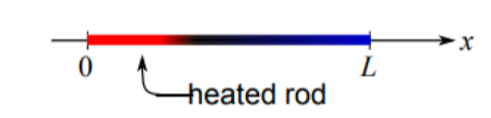
\includegraphics[scale=0.33]{rod.png}
\end{center}
\item The rod is said to be insulated at both ends and no internal heat sources or sinks are present.
\item An initial temperature profile of f(x) is assumed.
\end{enumerate}
\end{frame}

\begin{frame}{1-D Heat Equation}
\begin{enumerate}
\item Consider an arbitrary segment of the rod, whose width is $\Delta x$ and which is located at $x$.
\begin{center}
\begin{equation} \label{econserve}
	\dot{e}= \dot{q}_{left} - \dot{q}_{right}
\end{equation}
\end{center}
\begin{center}
\begin{equation} \label{four}
\dot{q} = -K_{0} \frac{\partial u}{\partial x}
\end{equation}
\end{center}
\item Fourier's law described in Equation~\ref{four} can be applied to find the fluxes on the left and right sides of the segment.
\begin{center}
\begin{equation} \label{cons-four}
c \rho A \Delta x \bigg(u(x+ \Delta x,t)-u(x,t) \bigg) = -K_{0} \Delta t A \bigg(  \Big( \frac{\partial u}{\partial x} \Big)_{x}-\Big( \frac{\partial u}{\partial x}\Big)_{x+ \Delta x} \bigg )
\end{equation}
\end{center}
\end{enumerate}
\end{frame}

\begin{frame}
\begin{enumerate}
\item Simplifying Equation~\ref{cons-four} leads to the 1D Heat equation which is a parabolic PDE.
\begin{center}
\begin{equation} \label{1diff}
\frac{\partial u}{\partial t}=\alpha \frac{\partial^{2} u}{\partial x^{2}}
\end{equation}
\end{center}
\item This equation is also known as the second order diffusion equation, the co-efficient $\alpha$ is known as the Thermal diffusivity and is a material property.
\item To make use of the Heat equation, Boundary conditions and Initial condition are required.
\item The initial condition in this case is the initial temperature profile $u(x,0)$.
\item The solution is effected by the boundary conditions which can be determined from the condition that the rod is insulated at both ends.
\end{enumerate}
\end{frame}

\section{Assumptions}
\begin{frame}{Initial and Boundary conditions}
\begin{enumerate}
\item At the boundaries, the rod is insulated at both ends i.e the heat flux at both ends is zero.
\begin{center}
	\begin{equation} \label{neumannbc}
\bigg( \frac{\partial u}{\partial x} \bigg)_{x=0} = \bigg( \frac{\partial u}{\partial x} \bigg)_{x=L} = 0
\end{equation}
\end{center}
\item This kind of boundary condition is known as the Neumann Boundary condition as opposed to holding the ends at a certain constant temperature which is known as the Dirichlet boundary condition. 
\begin{center}
\begin{equation} \label{u0}
u(x,0)=0.5 \big (  sin(x)+cos(x) \big )
\end{equation}
\end{center}
\item The Initial condition represented in Equation~\ref{u0} is a sinosuidal condition.
\end{enumerate}
\end{frame}

\begin{frame}{Material}
\begin{enumerate}
\item The thermal diffusivity $\alpha$ is a function of material properties.
\begin{center}
	\begin{equation} \label{alpha}
\alpha = \frac{K_{0}}{\rho c}
\end{equation}
\end{center}
\item \textbf{Aluminum} was chosen as the material of the rod, arbitrarily.
\item For this solution, iti is assumed that all the material properties are constant and do not vary with temperature.
\item The specific heat(c) of aluminum at STP is 0.91 $\frac{kJ}{kg-K}$.
\item The density($\rho$) of aluminum at STP is 2710 $\frac{kg}{m^{3}}$
\item The Thermal conductivity($K_{0}$) of Aluminum at STP is 205 $\frac{W}{m-K}$
\end{enumerate}
\end{frame}

\begin{frame}{Model}
\begin{enumerate}
\item The \textbf{Finite Difference Method} has been chosen to solve the problem as it is computationally least expensive and is suitable to solve parabolic PDEs with relatively simple boundary conditions.
\item The rod is divided into a grid of points at which function evaluations would be made.
\item The governing equation has been non-dimensionalized and the characteristic length $L$ is assumed to be of unit value.
\end{enumerate}
\end{frame}

\section{Numerical Scheme}

\begin{frame}{Crank Nicholson Scheme}
\begin{enumerate}
\item This scheme is semi-implicit in nature, as it involves matrix inversion while the previous timestep information is also considered as part of the solution.
\begin{center}
	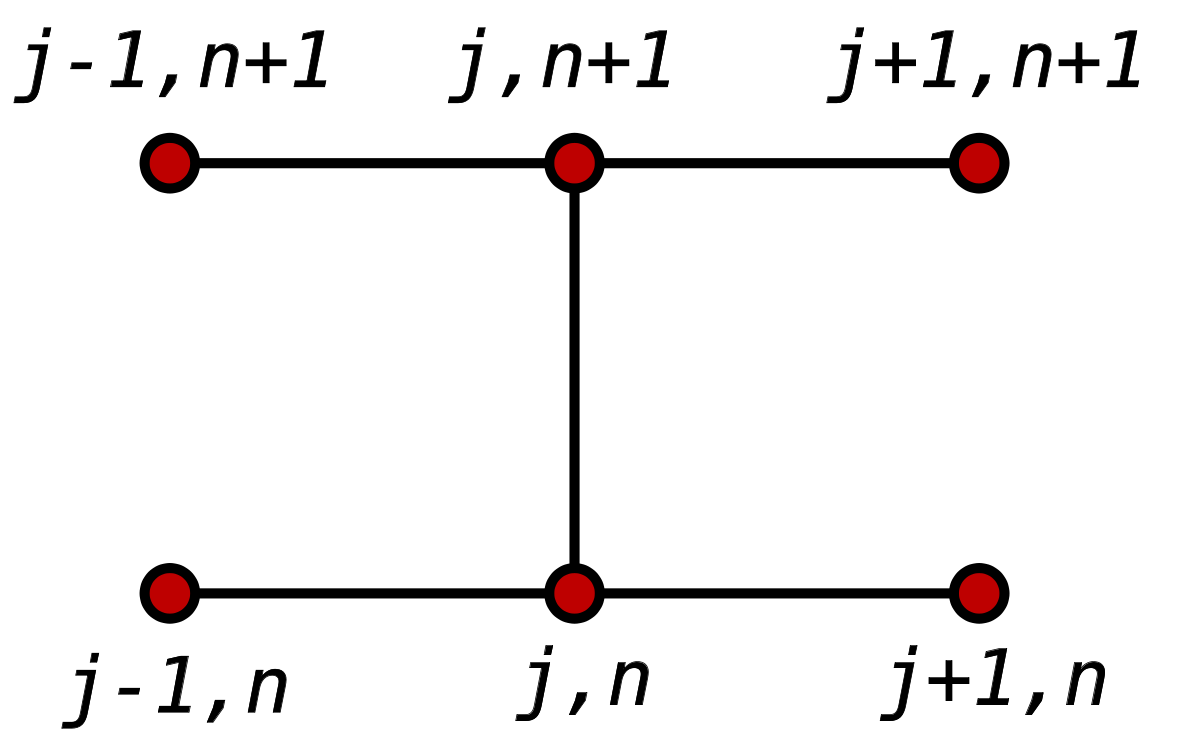
\includegraphics[scale=0.10]{stencil.png}
\end{center}
\item The scheme is second order accurate in space and time i.e $\mathcal{O}((\Delta x)^{2},(\Delta t)^{2})$.
\begin{center}
\begin{equation} \label{cfl}
\lambda = \frac{\alpha \Delta t}{(\Delta x)^{2}}
\end{equation}
\end{center}
\item It is unconditionally stable i.e for any value of the CFL number($\lambda$).
\end{enumerate}	
\end{frame}

\begin{frame}{Crank Nicholson Scheme}
\begin{enumerate}
\item The CN scheme is the most prominent of the Weighted Average schemes.
\begin{flalign*}
\Theta = 0.5 \\
u_{i}^{n+1}=u_{i}^{n}+ \lambda \bigg[ (1-\Theta)\Big(u_{i+1}^{n+1}-2u_{i}^{n+1}+u_{i-1}^{n+1} \Big)+ (\Theta)\Big(u_{i+1}^{n}-2u_{i}^{n}+u_{i-1}^{n} \Big) \bigg] 
\end{flalign*}
\begin{equation} \label{cn}
u_{i}^{n+1}=u_{i}^{n}+ \frac{\lambda}{2} \bigg[ \Big(u_{i+1}^{n+1}-2u_{i}^{n+1}+u_{i-1}^{n+1} \Big)+\Big(u_{i+1}^{n}-2u_{i}^{n}+u_{i-1}^{n} \Big) \bigg]  
\end{equation}
\item Equation~\ref{cn} can be represented in a matrix form as follows.
	\begin{equation} \label{cnvec}
\bm{A}u^{n+1} = \bm{B}u^{n}+\bm{b}
\end{equation}	
\end{enumerate}
\[
\bm{b}=\begin{bmatrix}
	2 \lambda \Delta x \dot{q}_{0} & \dots & \dots & \dots & \dots & \dots & \dots & 2 \lambda \Delta x \dot{q}_{L}
	\end{bmatrix}
\]
\end{frame}
\begin{frame}{Crank Nicholson Scheme}
\[
\bm{A} = \begin{bmatrix} 
	1+\lambda  & -\lambda & 0 & \dots & \dots &\dots & \dots & 0 \\
	\frac{- \lambda}{2} & 1+\lambda & \frac{- \lambda}{2} & \dots & \dots & \dots & \dots &  \vdots \\
	0  & \frac{- \lambda}{2}  & 1+\lambda & \frac{- \lambda}{2} & \dots & \dots & \dots & \vdots\\
	\vdots &  & \ddots & \ddots & \ddots & & & \vdots \\
	\vdots & & & \ddots & \ddots & \ddots & & \vdots \\
	\vdots & & & & \ddots & \ddots & -\lambda & 1+\lambda
    \end{bmatrix}
\]
\[
\bm{B} = \begin{bmatrix} 
        1-\lambda  & \lambda & 0 & \dots & \dots &\dots & \dots & 0 \\
        \frac{ \lambda}{2} & 1-\lambda & \frac{ \lambda}{2} & \dots & \dots & \dots & \dots &  \vdots \\
        0  & \frac{ \lambda}{2}  & 1-\lambda & \frac{ \lambda}{2} & \dots & \dots & \dots & \vdots\\
        \vdots &  & \ddots & \ddots & \ddots & & & \vdots \\
        \vdots & & & \ddots & \ddots & \ddots & & \vdots \\
        \vdots & & & & \ddots & \ddots & \lambda & 1-\lambda
    \end{bmatrix}
\]
\end{frame}
\begin{frame}{Crank Nicholson Scheme}
\begin{enumerate}
\item The scheme takes information from the present time step as well as the previous time step, making use of the maximum amount of information available.
\item However, the scheme does produce oscillations when the gradients are very high in the initial condition or during the first few time steps when this happens.
\item This is numerical dispersion is usually observed when the CFL Number ($\lambda$) is significantly higher than 0.5 and is caused by the presence of odd order terms in the modified PDE.
\end{enumerate}
\end{frame}

\begin{frame}{Rannacher Smoothing}
\begin{enumerate}
\item To avoid the dispersion caused by crank nicholson scheme, One strategy is to start the first two solutions with an implicit euler formulation and a timestep that is half the original value.
\item Implicit Euler scheme is also unconditionally stable and performs well even when gradients are high.
\item Implicit Euler scheme is first order in space and time i.e $\mathcal{O}((\Delta x),(\Delta t))$.
\item This implementation ensures that the high frequencies at the beginning of the solutio are damped out and then crank nicholson method which is much more accurate can take over.
\end{enumerate}
\end{frame}

\section{Algorithm}
\begin{frame}{Performance}
\begin{enumerate}
\item The entire project has been written in Python, with the numpy LinAlg solver to invert matrices.
\item The \textbf{np.linalg.solve()} function is of $\mathcal{O}(n^{3})$ which is the highest time complexity you will find in the algorithm.
\item On average, a solution with 2000 grid points over 500 time steps takes 28 seconds.
\item This implies that each matrix inversion is taking about 0.06 seconds.
\end{enumerate}
\end{frame}
\begin{frame}{Structure}
\begin{enumerate}
\item There are 6 python files that make up this project.
\begin{figure}
\begin{center}
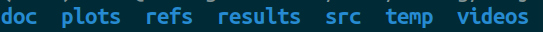
\includegraphics[scale=0.30]{dir.png}
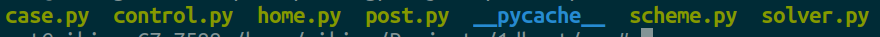
\includegraphics[scale=0.30]{srcdir.png}
\caption{The structure of the project and the source directory}
\label{dir}
\end{center}
\end{figure}
\item The solutions are solved in the \textbf{results} folder
\item The figures produced to create the video are saved in \textbf{temp}
\item The plots are docs are stored in their respective namesake folders.
\item The project is hosted on github and can be found \href{https://github.com/VishalKandala/1DiffCrank}{\textbf{here}}.
\end{enumerate}
\end{frame}

\begin{frame}{Setup}
\begin{enumerate}
	\item \textbf{control.py} contains all the control parameters such as the grid size, number of time steps and all the variables can be directly altered from here.
	\item \textbf{case.py} contains material property  information as well as the initial condition assumed in the problem, by editing this file, the entire solution can be changed.
	\item \textbf{scheme.py} contains the pre calculated co-efficient matrices \textbf{A},\textbf{B} and the vector \textbf{b} for both the Crank Nicholson scheme and the Implicit Euler scheme as both are used in the solution. 
\end{enumerate}
\end{frame}

\begin{frame}{function}
\begin{enumerate}
\item The user executes \textbf{home.py} with arguments "-s" and "-u0", these confirm whether a new solution must be generated and also which initial solution to apply. 
\item Here, based on the argument, if a new solution is to be generated, then the relevant parameters are pulled from control.py, case.py and scheme.py
\item The parameters are then input into a \textbf{solve()} function written in \textbf{solver.py} that saves csv results in results folder and returns a 2D array.
\item The solve() function implements Rannacher time stepping with co-efficients of CN scheme and implicit euler scheme that are pulled from scheme.py.
\item In home, this 2D array is passed on to the post processing functions present in \textbf{post.py}.
\end{enumerate}
\end{frame}

\section{Results}

\begin{frame}{Time Evolution of Solutions}
\begin{figure}
\begin{center}
	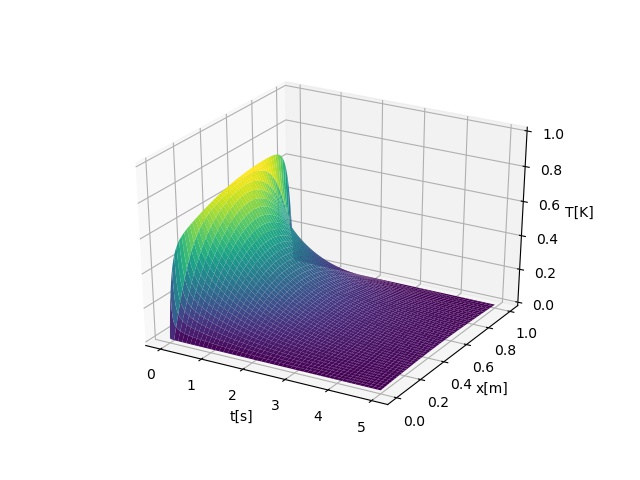
\includegraphics[scale=0.5]{../plots/evol2_0500_2000.jpg}
	\caption{Time evolution for u(x,0)=0.5(sin(x)+cos(x))}
	\label{fig:sin-cos-evol}
\end{center}
\end{figure}
\end{frame}

\begin{frame}{Time Evolution of Solutions}
\begin{figure}
\begin{center}
	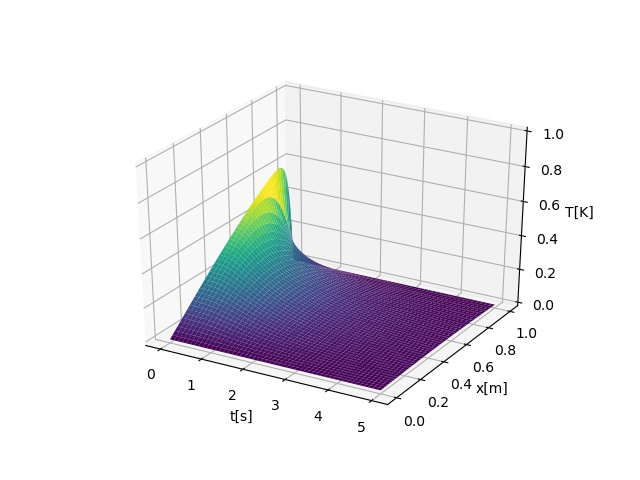
\includegraphics[scale=0.5]{../plots/evol0_0500_2000.jpg}
	\caption{Time evolution for u(x,0)=0.8(sin(x))}
	\label{fig:sin-evol}
\end{center}
\end{figure}
\end{frame}

\begin{frame}{Time Evolution of Solutions}
\begin{figure}
\begin{center}
	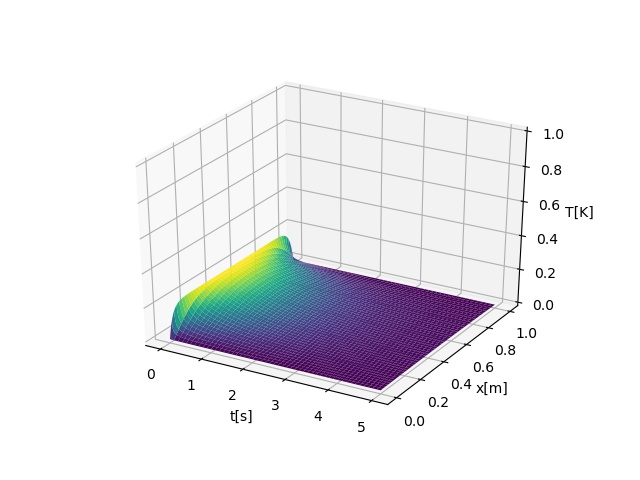
\includegraphics[scale=0.5]{../plots/evol1_0500_2000.jpg}
	\caption{Time evolution for u(x,0)=0.2 i.e constant}
	\label{fig:const-evol}
\end{center}
\end{figure}
\end{frame}

\begin{frame}{Snapshots of Solutions}
\begin{figure}
\begin{center}
	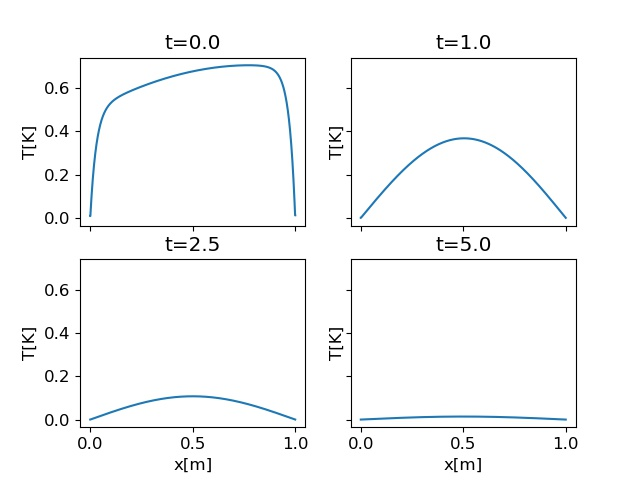
\includegraphics[scale=0.5]{../plots/snap_2_0500_2000.jpg}
	\caption{Snapshots of u(x,t) for  u(x,0)=0.5(sin(x)+cos(x))}
	\label{fig:sin-cos-snap}
\end{center}
\end{figure}
\end{frame}

\begin{frame}{Snapshots of Solutions}
\begin{figure}
\begin{center}
	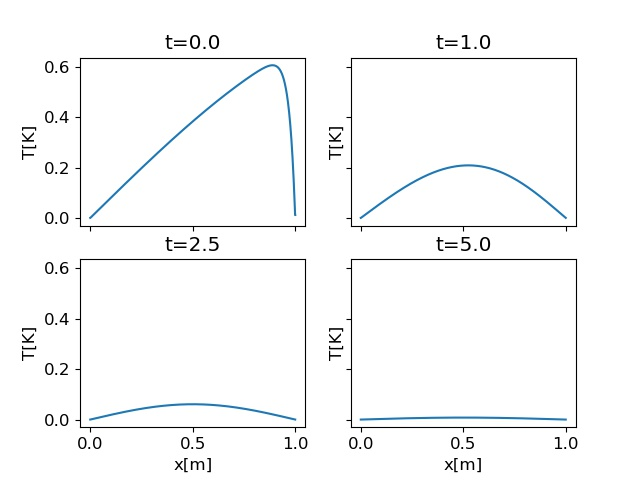
\includegraphics[scale=0.5]{../plots/snap_0_0500_2000.jpg}
	\caption{Snapshots of u(x,t) for u(x,0)=0.8(sin(x))}
	\label{fig:sin-snap}
\end{center}
\end{figure}
\end{frame}

\begin{frame}{Snapshots of Solutions}
\begin{figure}
\begin{center}
	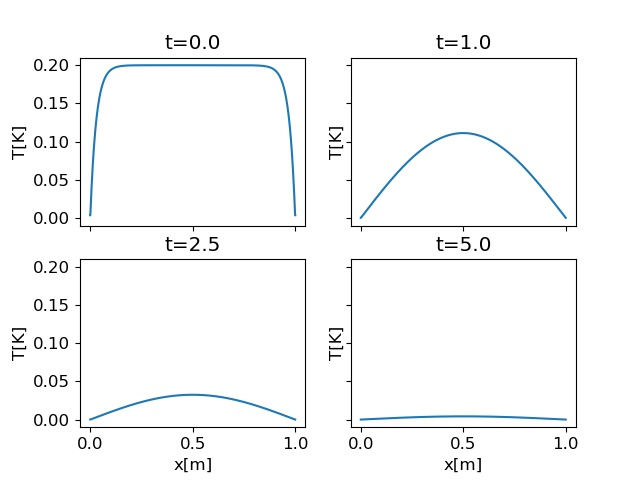
\includegraphics[scale=0.5]{../plots/snap_1_0500_2000.jpg}
	\caption{Snapshots of u(x,t) for u(x,0)=0.2 i.e constant}
	\label{fig:const-snap}
\end{center}
\end{figure}
\end{frame}

%\begin{frame}
%\frametitle{References}
%\footnotesize{
%\begin{thebibliography}{99} % Beamer does not support BibTeX so references must be inserted manually as below
%\bibitem[Smith, 2012]{p1} John Doe (2012)
%\newblock Title of the Publication
%\newblock \emph{Journal Name} 1(1), 11 -- 111.
%\end{thebibliography}
%}
%\end{frame}

%------------------------------------------------
\begin{frame}{}
\centering \Huge
	\emph{Thank You!}
\end{frame}

\end{document}
